% copied from the thesis chapter on fairness (content/fairness/fairness.tex, lines 1204-1351)
\begin{figure}[!hbp]
\centering
\begin{subfigure}{0.8\textwidth}
\begin{center}
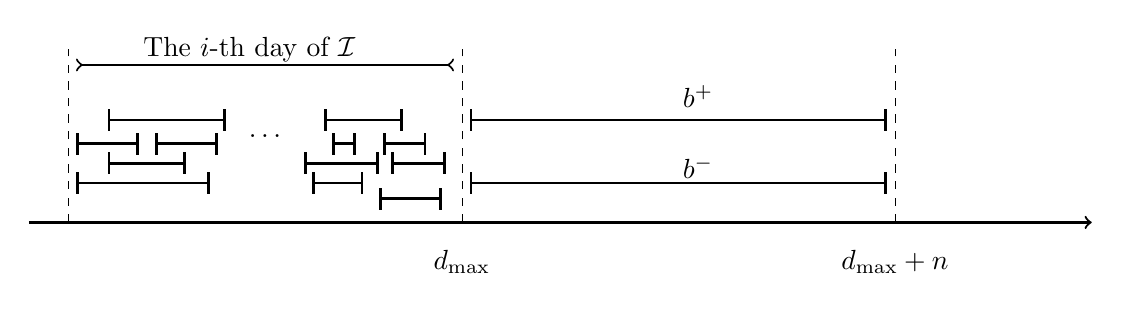
\begin{tikzpicture}

    \def\dmax{5.5}
    \def\eps{.1}
    % main axis
    \draw[thick,->] (0,0) -- (13.5,0) node[anchor=north west] {};
    % I dashed borders
    \draw[line width=0.1, dashed]
    (\dmax,-.) -- (\dmax,2.2) node[anchor=north] {};
    \node at (({\dmax}, -.5) {$d_{\max}$};
    \draw[line width=0.1, dashed]
    (0.5,-.) -- (0.5,2.2) node[anchor=north] {};
    \node at (({11.}, -.5) {$d_{\max}+n$};
    
    \draw[line width=0.1, dashed]
    (11.,-.) -- (11.,2.2) node[anchor=north] {};

    % I
    \draw[line width=.75, >-<]
  ({0.5+\eps}, 2.) -- ({\dmax-\eps}, 2.) node[anchor=north west] {};
  \node at (({\dmax*0.5+\eps*0.5}, 2.2) {The $i$-th day of $\mathcal{I}$};
    
    % I intervals

    \node at (({\dmax*0.5+0.25}, 1.1) {$\dots$};
  \draw[line width=1, |-|]
  ({0.5+\eps}, .5) -- ({2.3}, .5) node[anchor=north west] {};
  \draw[line width=1, |-|]
  ({0.5+\eps}, 1.) -- ({1.5-\eps}, 1.) node[anchor=north west] {};
  \draw[line width=1, |-|]
  ({1.5+\eps}, 1.) -- ({2.5-\eps}, 1.) node[anchor=north west] {};
  \draw[line width=1, |-|]
  (1, .75) -- ({2.}, .75) node[anchor=north west] {};
  \draw[line width=1, |-|]
  (1, 1.3) -- ({2.5}, 1.3) node[anchor=north west] {};
  \draw[line width=1, |-|]
  (1, 1.3) -- ({2.5}, 1.3) node[anchor=north west] {};


\draw[line width=1, |-|]
  (\dmax*0.5+1.7, .3) -- ({\dmax*0.5+2.5}, .3) node[anchor=north west] {};
  \draw[line width=1, |-|]
  ({\dmax*0.5+0.75+\eps}, .5) -- ({\dmax*0.5+1.5}, .5) node[anchor=north west] {};
  \draw[line width=1, |-|]
  ({\dmax*0.5+1.75+\eps}, .75) -- ({\dmax*0.5+2.65-\eps}, .75) node[anchor=north west] {};
  \draw[line width=1, |-|]
  (\dmax*0.5+.75, .75) -- ({\dmax*0.5+1.7}, .75) node[anchor=north west] {};
    \draw[line width=1, |-|]
  ({\dmax*0.5+1.+\eps}, 1.) -- ({\dmax*0.5+1.5-\eps}, 1.) node[anchor=north west] {};
    \draw[line width=1, |-|]
  ({\dmax*0.5+1.65+\eps}, 1.) -- ({\dmax*0.5+2.4-\eps}, 1.) node[anchor=north west] {};
  \draw[line width=1, |-|]
  (\dmax*0.5+1, 1.3) -- ({\dmax*0.5+2.}, 1.3) node[anchor=north west] {};


   \draw[line width=1, |-|]
  (\dmax+\eps, 1.3) -- ({11.-\eps}, 1.3) node[anchor=north west] {};
  \node at (({8.5}, 1.6) {$b^+$};
   \draw[line width=1, |-|]
  (\dmax+\eps, .5) -- ({11.-\eps}, .5) node[anchor=north west] {};
  \node at (({8.5}, .7) {$b^-$};
  
    \end{tikzpicture}
    \caption{When $1\leq i\leq \q$, the jobs of the original clients have the same intervals as in  the $i$-th day of $\mathcal{I}$.}
    \end{center}
    \end{subfigure}

  
% \end{tikzpicture}
 \begin{subfigure}{0.8\textwidth}
        \begin{center}
            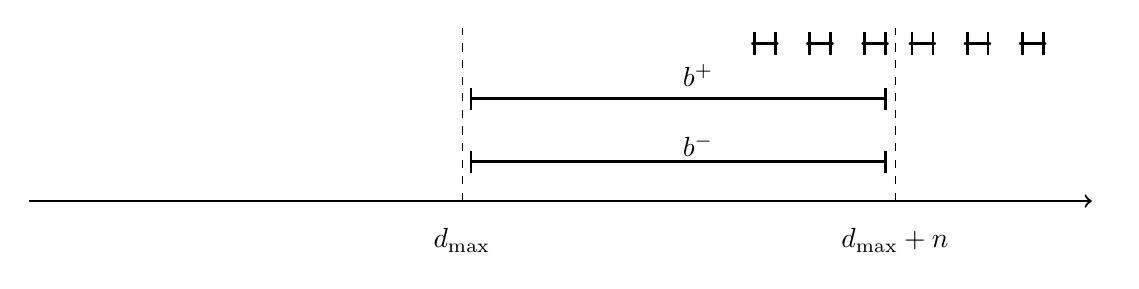
\begin{tikzpicture}

                 \def\dmax{5.5}
    \def\eps{.1}
    % main axis
    \draw[thick,->] (0,0) -- (13.5,0) node[anchor=north west] {};
    % I dashed borders
    \draw[line width=0.1, dashed]
    (\dmax,-.) -- (\dmax,2.2) node[anchor=north] {};
    \node at (({\dmax}, -.5) {$d_{\max}$};
    \node at (({11.}, -.5) {$d_{\max}+n$};
    \draw[line width=0.1, dashed]
    (11.,-.) -- (11.,2.2) node[anchor=north] {};

    
   \draw[line width=1, |-|]
  (\dmax+\eps, 1.3) -- ({11.-\eps}, 1.3) node[anchor=north west] {};
  \node at (({8.5}, 1.6) {$b^+$};
   \draw[line width=1, |-|]
  (\dmax+\eps, .5) -- ({11.-\eps}, .5) node[anchor=north west] {};
  \node at (({8.5}, .7) {$b^-$};


% Intervals over b^- b^+
\foreach \x/\i in
    {
        1/1,2/3,3/1
    }
    {
        \ifthenelse{\i = 0}{
        
        }{
         \ifthenelse{\i = 1}{
                \draw[line width=1, |-|]
                  (\dmax+3+\x*0.7, 2) -- ({\dmax+3+\x*0.7+0.3}, 2) node[anchor=north west] {};
         }{

            \node at (\dmax+3+\x*0.7+0.15, 2) {$\dots$};
         
         }
        }

    }  

% Intervals after b^- b^+
\foreach \x/\i in
    {
        1/1,2/3,3/1
    }
    {
        \ifthenelse{\i = 0}{
        
        }{
         \ifthenelse{\i = 1}{
                \draw[line width=1, |-|]
                  (10.5+\x*0.7, 2) -- ({10.5+\x*0.7+0.3}, 2) node[anchor=north west] {};
         }{

            \node at (10.5+\x*0.7+0.15, 2) {$\dots$};
         
         }
        }

    }  
    
   
\end{tikzpicture}
\caption{When $\q< i\leq2\q$ let the jobs of original clients either intersect the jobs of both $b^-$ and $b^+$  (for $\{\ c\ |\ i-\q \leq k_c\ \}$) \textit{or} intersect no jobs at all (for $\{\ c\ |\ i-\q > k_c\ \}$).}
\end{center}
\end{subfigure}
\caption{An intersection model of the $i$-th day's jobs.}
\label{fig:reduction-unweighted}
\end{figure}
